\chapter{Υλοποίηση Αρχιτεκτονικής}
\label{chap:Impl}

\section{Εισαγωγή}

Η υλοποίηση της προτεινόμενης αρχιτεκτονικής έγινε με τη χρήση 
της γλώσσας προγραμματισμού Java. Όπως έχει αναφερθεί η Guice 
χρησιμοποιήθηκε για την υποστήριξη του προτύπου dependency injection. Η 
υλοποίηση της CORBA που προσφέρεται από την Java καλύπτει τις ανάγκες 
απομακρυσμένων κλήσεων συναρτήσεων. Η ανάγκη καταγραφής μηνυμάτων 
καλύφθηκε από την βιβλιοθήκη log4j και της slf4j. Τέλος, για την 
διενέργεια ελέγχων χρησιμοποιήθηκε η βιβλιοθήκη JUnit.

Έγινε χρήση διάφορων εργαλείων όπως το Ant το οποίο καθοδηγεί 
μεταγλώττιση, την εκτέλεση των unit test, την εξαγωγή της τεκμηρίωσης 
μέσω javadoc και την δημιουργία της βιβλιοθήκης ως jar αρχείου. Αναγκαία 
ήταν διάφορα εργαλεία στατικής ανάλυσης του κώδικα που προσφέρονταν μέσω 
του IDE IntelijIDEA. Για την διαχείριση του κώδικα και των εκδόσεων του 
χρησιμοποιήθηκε το git. Ο κώδικας της βιβλιοθήκης υπάρχει στο αποθετήριο 
\url{https://github.com/Archimidis/pgrid}

\section{Common Object Request Broker Architecture (CORBA)}

Η υλοποίηση βασίστηκε πάνω στην CORBA 
\citep{CorbaSpec, CorbaSpecP1, CorbaSpecP2, CorbaSpecP3} για 
την επικοινωνία των peer μέσω κλήσεων απομακρυσμένων συναρτήσεων (rpc). 
Η δομή της αρχιτεκτονικής της δε μας αφορά. Είναι σημαντικές, όμως, 
κάποιες λεπτομέρειες οι οποίες αφορούν την περαιτέρω παραμετροποίηση του 
συστήματος. 

Για την υλοποίηση των υπηρεσιών πρέπει να γραφεί σε idl η περιγραφή 
αυτής. Μέσω της idl παράγονται ο κώδικας που είναι χρήσιμος για την 
κλήση μιας συνάρτησης client (stub code) και ο κώδικας για την 
εξυπηρέτηση αυτών των κλήσεων (skeleton code). Το δεύτερο κομμάτι είναι 
εκεί όπου υλοποιείται η λειτουργικότητα της διεπαφής. Η προώθηση των 
κλήσεων σε αυτό γίνεται μέσω του servant.

Ένα σημαντικό κομμάτι της αρχιτεκτονικής που ενδιαφέρει και εμάς είναι ο 
Portable Object Adapter (POA). Ο ρόλος του είναι να ενώσει τους servant 
με το ORB και η διαχείριση του περιβάλλοντος το αντικείμενο που είναι η 
υλοποίηση της διεπαφής κατά τον χρόνο εκτέλεσης. Μέσω αυτού γίνεται η 
αντιστοίχιση servant με υλοποιήσεις. Επίσης, ο POA μπορεί να 
ενεργοποιήσει το αντικείμενο και η προσαρμογή του σε συγκεκριμένες 
πολιτικές. Το τελευταίο είναι που προσθέτει επιπλέον δυνατότητες 
παραμετροποίησης του συστήματος.

Οι πολιτικές που χρησιμοποιούνται από τον POA είναι οι παρακάτω 
\citep{CorbaProg2001}:

\newcounter{numberedCntBC}
\begin{enumerate}
\item \textbf{Μοναδικότητα ID.} Καθορίζει αν περισσότερα από ένα ID 
αντικειμένου θα αναφέρεται στον ίδιο servant.
\item \textbf{Ανάθεση ID.} Καθορίζει αν την ανάθεση των ID την κάνει ο 
POA ή ο προγραμματιστής.
\item \textbf{Διάρκεια ζωής.} Καθορίζει αν τα αντικείμενα είναι 
παροδικά ή μόνιμα. Αν το αντικείμενο, δηλαδή, είναι προσιτό μετά την 
καταστροφή του POA ή όχι.
\item \textbf{Διατήρηση servant.} Καθορίζει αν ο POA κρατά τις 
συσχετίσεις μεταξύ ID αντικειμένου και servant σε μια δομή που 
ονομάζεται Active Object Map. Σε αντίθετη περίπτωση στηρίζεται στον 
προεπιλεγμένο servant ή σε servant locator για τον εντοπισμό του 
κατάλληλου servant με στόχο την εξυπηρέτηση της αίτησης.
\item \textbf{Επεξεργασία αίτησης.} Καθορίζει αν ο POA χρησιμοποιεί 
είτε μόνο το Active Object Map, είτε μόνο τον προεπιλεγμένο servant είτε 
την χρήση του servant manager. Η επιλογή που θα γίνει για την διατήρηση 
του servant επηρεάζει και τον τρόπο με τον οποίο θα γίνει η επεξεργασία. 
Συγκεκριμένα για τον servant manager υπάρχουν δυο κατηγορίες
\begin{itemize}
\item \textbf{Servant activator.} βάσει αυτού δημιουργείται ο servant 
και όταν τελειώσει ο κύκλος ζωής του τότε καταστρέφεται.
\item \textbf{Servant locator.} Εύρεση του κατάλληλου servant ο οποίος 
δεν είναι καταχωρημένος στο Active Object Map.
\end{itemize}
\item \textbf{Πολιτική νημάτων.} Καθορίζει αν θα ακολουθηθεί 
μονονηματική πολιτική ή όχι.
\item \textbf{Σιωπηρή ενεργοποίηση servant.} Καθορίζει αν ο POA μπορεί 
να ενεργοποιήσει έναν servant όταν μια αναφορά προς ένα ID δημιουργηθεί.
\setcounter{numberedCntBC}{\theenumi}
\end{enumerate}
Μπορούν συνδυασμοί μπορούν να προκύψουν από τα παραπάνω. Η χρήση μόνο 
του Active Object Map για την επεξεργασία των αιτήσεων συνοδεύεται με 
την επιλογή της αποθήκευσης αντιστοιχίσεων ID και servant σε αυτόν. 
Πρέπει να γνωρίζουμε πριν την εκκίνηση του συστήματος τον αριθμό των 
servant αφού αυτοί θα δημιουργηθούν και θα εγκατασταθούν ρητά.

Στην περίπτωση που ο αριθμός των αντικειμένων είναι μεγάλος ή δεν τον 
γνωρίζουμε εξ αρχής τότε είναι χρήσιμος ο servant manager. Αν επιλέξουμε 
την ύπαρξη αντιστοιχίσεων στο Active Object Map, τότε χρησιμοποιείται ο 
servant activator. Αν δεν βρεθεί ένα αντικείμενο μέσω του ID του τότε 
ενεργοποιείται ο κατάλληλος servant. Σε αντίθετη περίπτωση όπου δεν 
έχουμε Active Object Map τότε χρησιμοποιείται ο servant locator. Ο 
servant επιτρέπει την παροχή διαφορετικών servant που αντιστοιχούν σε 
διαφορετικές υλοποιήσεις της διεπαφής που καλείται.

Συνεπώς, παρέχοντας υλοποιήσεις των servant manager μπορούμε να 
καθορίσουμε περαιτέρω τον κύκλο ζωής των υπηρεσιών και των αντικειμένων 
που χρησιμοποιούν ανάλογα με τις απαιτήσεις του περιβάλλοντος στο οποίο 
εκτελείται ο peer.

\section{Επίπεδο Οντοτήτων - Entity Layer}

Όπως έχει αναφερθεί στο επίπεδο οντοτήτων υπάρχει οτιδήποτε 
αποθηκεύει κατάσταση ή δεδομένα και παρέχει πρόσβαση σε υπηρεσίες που 
προσφέρει το λειτουργικό σύστημα πάνω στο οποίο εκτελείται η εφαρμογή.

Ένας peer για να περιγραφεί ολοκληρωμένα χρειάζεται η διεύθυνσή 
του (ip και port). Επίσης, μετά την εισαγωγή του στο δίκτυο είναι 
υπεύθυνος για ένα κομμάτι του χώρου κλειδιών το οποίο καθορίζεται από το 
μονοπάτι που του έχει δοθεί. Χρειάζεται και αυτή η πληροφορία. Τέλος, 
κάθε peer αναγνωρίζεται μοναδικά από ένα UUID που του δίνεται κατά την 
εκκίνησή του. Τα παραπάνω περιγράφονται από την διεπαφή Host.

Δίνονται διεπαφές που αναπαριστούν ένα κλειδί, Key, καθώς και ενός 
πεδίου κλειδιών, KeyRange, του συστήματος. Τα κλειδιά όπως έχει 
αναφερθεί συσχετίζονται είτε με peer είτε με πόρους που προσφέρονται από 
τους peer στο δίκτυο. Επίσης, προσφέρεται διεπαφή που αφορά τα μονοπάτια 
του p-grid δέντρου, PGridPath. Διαφορετική σημασιολογία ή αναπαράσταση 
σε όλα τα παραπάνω μπορεί να δοθεί επεκτείνοντας αυτές τις διεπαφές. Η 
παραγωγή αντικειμένων αυτών των τύπων για χρήση από τον χρήστη γίνεται 
μέσω του σχεδιαστικού προτύπου factory \citep{GoF}.

Η έννοια του χρόνου σε ένα κατανεμημένο σύστημα είναι σημαντική για την 
σειριοποίηση των γεγονότων που συμβαίνουν σε αυτό. Υπάρχει η έννοια του 
ρολογιού στην διεπαφή PeerClock και δίνεται επίσης η κλασική υλοποίηση 
των Lamport ρολογιών \citep{Lamport}. Η υλοποίηση είναι ασφαλής για σε 
πολυνηματικό κώδικα.

Κάθε peer που μετέχει στο δίκτυο αποθηκεύει αναφορές προς άλλους 
peer. Ο τρόπος και η δομή με την οποία αποθηκεύονται αυτές εκφράζονται 
μέσω του πίνακα δρομολόγησης, RoutingTable. Η παραγωγή αντικειμένων 
αυτού του τύπου επιτυγχάνεται με τη χρήση του σχεδιαστικού προτύπου 
abstract factory \citep{GoF}. Η υλοποίηση που παρέχεται για τον 
πίνακα δρομολόγησης είναι ασφαλής για χρήση σε πολυνηματικό κώδικα, 
δεδομένης της ταυτόχρονης χρήσης από πολλές υπηρεσίες.

Η επικοινωνία μεταξύ των peer του δικτύου επιτυγχάνεται μέσω 
απομακρυσμένων κλήσεων συναρτήσεων (rpc). Αυτή η 
λειτουργικότητα προσφέρεται από την CORBA. Ως οντότητα θεωρείται το ORB 
και επιπλέον για την ρύθμισή του και την παραγωγή του κατά την εκκίνηση 
του peer χρησιμοποιείται abstract factory. Κάθε ORB είναι μοναδικό για 
κάθε peer και πρέπει να υπάρχει ένα αντικείμενο αυτού του τύπου ανά 
εφαρμογή.

Στην \ref{fig:EntityLayer} φαίνεται το UML διάγραμμα κλάσεων που αφορά 
το επίπεδο οντοτήτων. Η κλάση EntityModyle περιέχει την παραμετροποίηση 
που απαιτείται από την Guice.

\begin{figure}[htbp]
  \begin{center}
    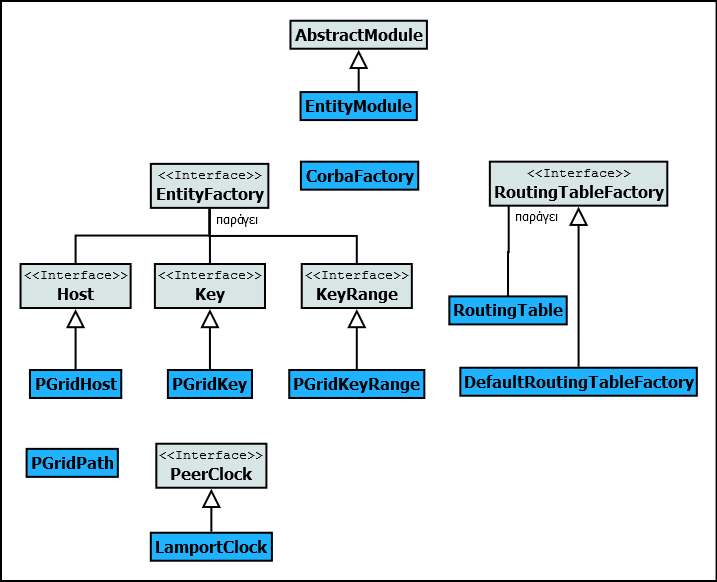
\includegraphics[width=0.9\textwidth]{Figures/Architecture/Entity_Layer/EntityLayer_ClassDiagram.png}
  \end{center}
  \caption{Διάγραμμα κλάσεων επιπέδου οντοτήτων}
  \label{fig:EntityLayer}
\end{figure}

\section{Επίπεδο Υπηρεσιών - Service Layer}

Στο επίπεδο των υπηρεσιών υπάρχουν όλα τα πρωτόκολλα που 
προσφέρει το σύστημα εκφρασμένα ως υπηρεσίες. Στην παρούσα φάση της 
υλοποίησης έχουμε το πρωτόκολλο Exchange και αυτό της ανοχής λαθών 
Repair, όπως αυτά έχουν περιγραφεί. Επίσης, έχει υλοποιηθεί μια υπηρεσία 
που αφορά την προσομοίωση του συστήματος και βοηθά στον έλεγχό του. Στις 
επόμενες ενότητες θα αναλυθούν οι υλοποιήσεις των προαναφερθέντων. 
Παρέχεται, επίσης και μια υπηρεσία για την αρχικοποίηση του συστήματος.

Στο διάγραμμα συστατικών (component) \ref{fig:ServiceComponents} 
φαίνονται οι μονάδες του επιπέδου. Το επίπεδο περιλαμβάνει τα module 
των υπηρεσιών Exchange, Repair, Simulation και αρχικοποίησης. Επίσης, 
φαίνονται οι τρεις διεπαφές που εκτίθενται στα ανώτερα επίπεδα καθώς και 
οι εξαρτήσεις του παρόντος από το επίπεδο οντοτήτων. Επίσης, κάθε υπηρεσία 
έχει ανάγκη το ORB για επικοινωνία και τον πίνακα δρομολόγησης του τοπικού 
peer. Αυτά αποθηκεύονται στην κλάση LocalPeerContext. Κάθε κατά την διάρκεια 
εκτέλεσης του συστήματος, υπάρχει μόνο αντικείμενο αυτής της κλάσης το 
οποίο επιστρέφεται από την Guice.

\begin{figure}[htbp]
  \begin{center}
    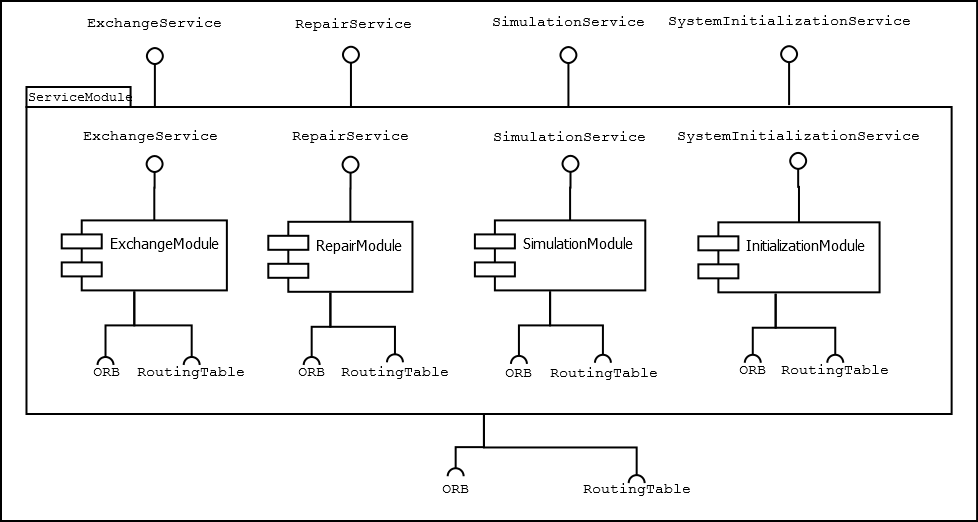
\includegraphics[width=0.9\textwidth]{Figures/Architecture/Service_Layer/Service_ComponentDiagram.png}
  \end{center}
  \caption{Διάγραμμα συστατικών επιπέδου υπηρεσιών}
  \label{fig:ServiceComponents}
\end{figure}

\subsection{Υλοποίηση Πρωτοκόλλου Exchange ως Υπηρεσία}

\begin{figure}[htbp]
  \begin{center}
    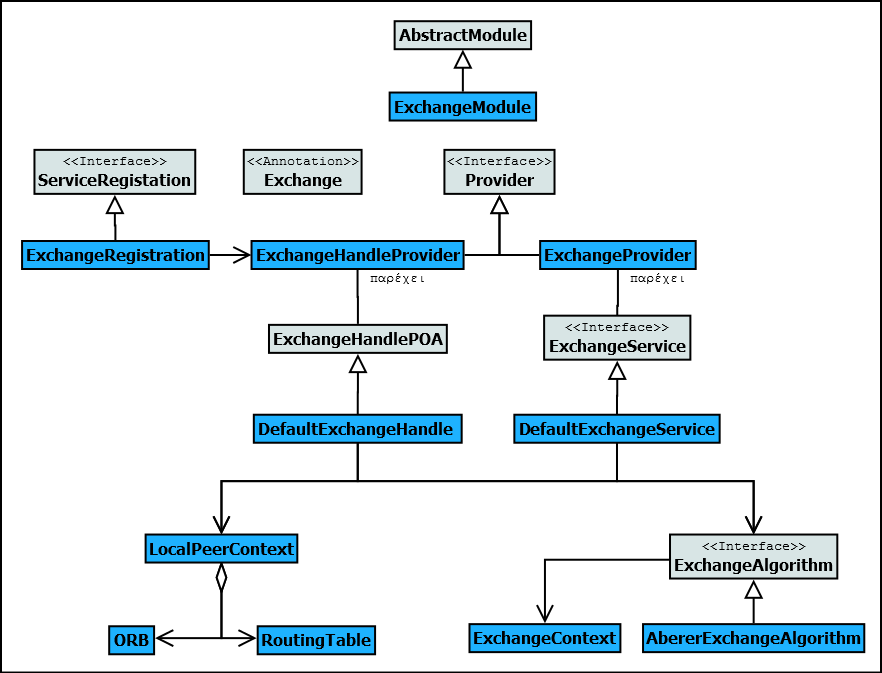
\includegraphics[width=0.9\textwidth]{Figures/Architecture/Service_Layer/ExchangeService_ClassDiagram.png}
  \end{center}
  \caption{Διάγραμμα κλάσεων υπηρεσίας Exchange}
  \label{fig:ExhangeService}
\end{figure}

Στην εικόνα \ref{fig:ExhangeService} φαίνεται το διάγραμμα κλάσεων της 
υπηρεσίας Exchange. Η δομή της ακολουθεί την γενική δομή της υπηρεσίας που 
περιγράφηκε σε προηγούμενη ενότητα. 

Η διεπαφή που εκθέτει την λειτουργικότητα της υπηρεσίας στο επίπεδο των 
διεργασιών και της εφαρμογή είναι η ExchangeService. Με την κλήση της 
μεθόδου που προσφέρει, ο τοπικός peer επικοινωνεί με τον απομακρυσμένο 
peer που έχει δοθεί ως όρισμα και εκτελούν τον αλγόριθμο exchange. Στην 
περίπτωση όπου υπάρχει πρόβλημα κατά την επικοινωνία, αν παράδειγμα ο 
απομακρυσμένος peer έχει αποτύχει, η υπηρεσία τερματίζει χωρίς να 
εκτελέσει τον αλγόριθμο με ένα CommunicationException.

Αντίστοιχα, για την πλευρά του εξυπηρετητή του peer που αφορά την CORBA 
έχουμε την κλάση ExchangeHandlePOA που έχει παραχθεί μέσω της idl. 
Παρέχει την υλοποίηση του CORBA αντικειμένου η οποία θα εγκατασταθεί 
στην CORBA και θα μπορεί να εξυπηρετεί απομακρυσμένες αιτήσεις εκτέλεσης 
του αλγορίθμου.

Οι παραπάνω διεπαφές έχουν μια προεπιλεγμένη υλοποίησης. Αυτές 
σχετίζονται με την διεπαφή ExchangeAlgorithm και της υλοποίησης της, την κλάση 
AbererExchangeAlgorithm. Η μέθοδος που προσφέρει δέχεται ένα αντικείμενο 
τύπου ExchangeContext. Το ExchangeContext περιέχει όλη την πληροφορία 
που χρειάζεται, όπως ο πίνακας δρομολόγησης, για να εκτελεστεί ο 
αλγόριθμος.

Για την κατασκευή αντικειμένων των τύπων που δηλώνονται από τις διεπαφές 
ExchangeService και ExchangeHandlePOA υλοποιείται η διεπαφή Provider. Ο 
ExchangeProvider παρέχει νέα αντικείμενα της ExchangeService σε κάθε 
αίτηση παροχής. 

Αρχικοποιεί την υπηρεσία με όλα τα απαραίτητα αντικείμενα και σταθερές 
όπως ο μέγιστος αριθμός αναδρομών που θα εκτελεστεί ο αλγόριθμος. 
Αντίστοιχα για την ExchangeHandlePOA έχουμε τον ExchangeHandleProvider, 
μόνο που εδώ παρέχεται πάντα το ίδιο αντικείμενο σε κάθε αίτηση.

Για την εγκατάσταση της υπηρεσίας στην CORBA έχουμε την υλοποίηση της 
διεπαφής ServiceRegistration, την ExchangeRegistration. Για να 
διευκρινιστεί στην Guice ποια υλοποίηση της ServiceRegistration θέλουμε, 
έχουμε το Annotation Simulation.

Τέλος, η όλη σύνδεση διεπαφών και υλοποιήσεων καθώς και τον καθορισμό 
του κύκλου ζωής των αντικειμένων βρίσκεται στην κλάση ExchangeModule.

\subsection{Υλοποίηση Πρωτοκόλλου Repair ως Υπηρεσία}

\begin{figure}[htbp]
  \begin{center}
    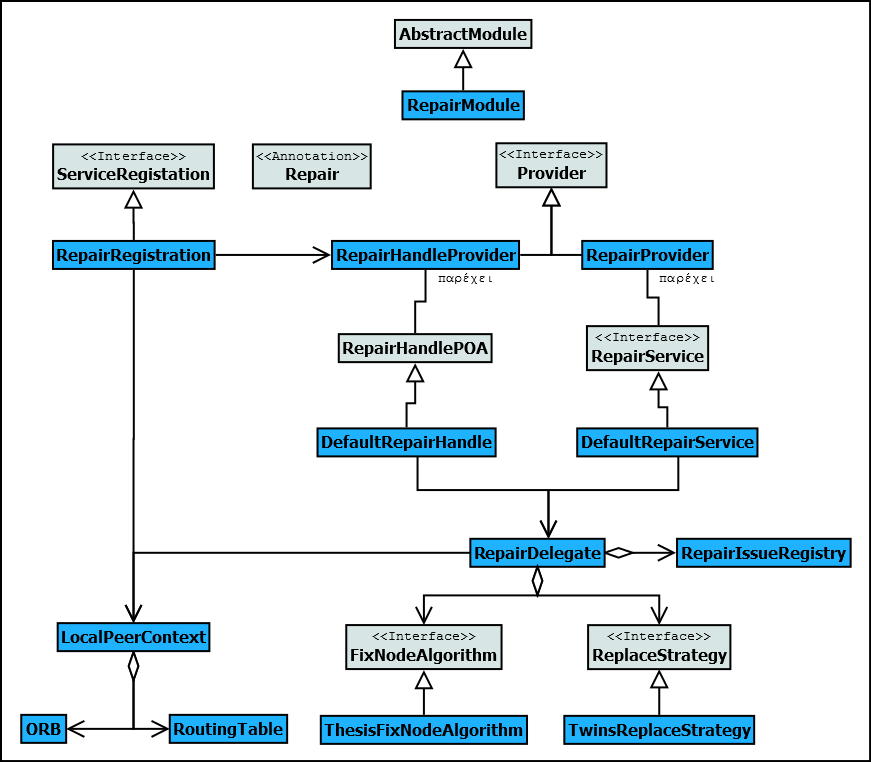
\includegraphics[width=\textwidth]{Figures/Architecture/Service_Layer/RepairService_ClassDiagram.png}
  \end{center}
  \caption{Διάγραμμα κλάσεων υπηρεσίας Repair}
  \label{fig:RepairService}
\end{figure}

Στην εικόνα \ref{fig:RepairService} φαίνεται το διάγραμμα κλάσεων της υπηρεσίας 
Repair. Αντίστοιχα με το γενικό μοντέλο της υπηρεσίας έχουμε τις 
διεπαφές RepairService και RepairHandlePOA. 

Η διεπαφή RepairService αφορά τις διεργασίες και την εφαρμογή. 
Προσφέρονται δυο μέθοδοι επιδιόρθωσης στην περίπτωση ενός αποτυχημένου 
peer ή την περίπτωση ενός αποτυχημένου υποδέντρου του δικτύου. Μετά το 
πέρας εκτέλεσης της υπηρεσίας θα έχει διορθωθεί το λάθος ή οποιοδήποτε 
αποτυχία ανακαλυφθεί στην πορεία.

Η διεπαφή RepairHandlePOA αφορά την CORBA και παράγεται μέσω της idl. Η 
υλοποίηση της φροντίζει για την αποδοχή απομακρυσμένων αιτήσεων και 
συνέχισης του αλγορίθμου.

Εδώ ακολουθούμε διαφορετική τακτική από αυτή της υπηρεσίας Exchange. Για 
την αποφυγή διπλοποίησης λειτουργικότητας και της επανάληψης κώδικα σε 
πολλά σημεία (αρχή DRY \citep{Pragmatic1999} ), 
έχουμε την κλάση RepairDelegate. Σε αυτήν αναφέρονται οι υλοποιήσεις των 
διεπαφών RepairService και RepairHandlePOA για την εξυπηρέτηση των 
αιτήσεων που δέχονται. 

Παρέχονται δυο διεπαφές που αφορούν η μια τον αλγόριθμο \ref{algo:Continuation} 
FindContinuation και η άλλη την τελική διόρθωσης του προβλήματος 
από τον αλγόριθμο \ref{algo:Replace} Replace όπως έχει προκύψει από την 
ανάλυση του πρωτοκόλλου ανοχής λαθών στην ενότητα \ref{sec:Fault}. 
Και οι δυο ακολουθούν το σχεδιαστικό πρότυπο Strategy \citep{GoF}.

Συνολικά, η διεπαφή FindContinuationAlgorithm καθορίζει την κατεύθυνση που 
πρέπει να πάρει αλγόριθμος διασχίζοντας την τοπολογία του δικτύου, 
επιστρέφοντας τον κατάλληλο peer. Η διεπαφή ReplaceStrategy, 
χρησιμοποιείται όταν ο αλγόριθμος έχει καταλήξει στους δυο peer που θα 
λύσουν την αποτυχία. Η κλάση RepairDelegate περιέχει όλη την λογική που 
αφορά την επικοινωνία μεταξύ των peer για την λύση του προβλήματος. 
Επίσης, κατά την εκτέλεση της υπηρεσίας μπορεί να ανακαλυφθούν 
αποτυχημένοι peer. Κάθε ανακάλυψη αποτυχίας καταχωρείται στην 
RepairRegistry. Η RepairDelegate ελέγχει αν μπορούν να γενικευθούν 
κάποια προβλήματα από μεμονωμένους αποτυχημένους peer σε ολόκληρα 
αποτυχημένα υπόδεντρα και να καθοδηγήσει την εκτέλεση σε λύση 
υποδέντρου.

Για την κατασκευή αντικειμένων των κλάσεων που υλοποιούν τις διεπαφές 
RepairService και RepairHandlePOA υλοποιείται ο Provider. Ο RepairProvider 
προσφέρει νέα αντικείμενα τύπου RepairService σε κάθε αίτηση παροχής. 
Αντίστοιχα ο RepairHandleProvider προσφέρει το ίδιο αντικείμενο τύπου 
RepairHandlePOA. Κατά την κατασκευή και των δυο παραπάνω τύπων 
χρησιμοποιείται το ίδιο αντικείμενο τύπου RepairRegistry.

Έχουμε την υλοποίηση της διεπαφής ServiceRegistration, 
RepairRegistration, για την εγκατάσταση της υπηρεσίας την CORBA καθώς 
και το Annotation Repair χρήσιμο στην Guice.

Στην κλάση RepairModule έχουμε την παραμετροποίηση της 
υπηρεσίας, την συσχέτιση διεπαφών και υλοποιήσεων όπως φαίνονται στο 
διάγραμμα κλάσεων και την δήλωση του κύκλου ζωής των αντικειμένων.

\subsection{Υλοποίηση Υπηρεσίας Προσομοίωσης}

\begin{figure}[htbp]
  \begin{center}
    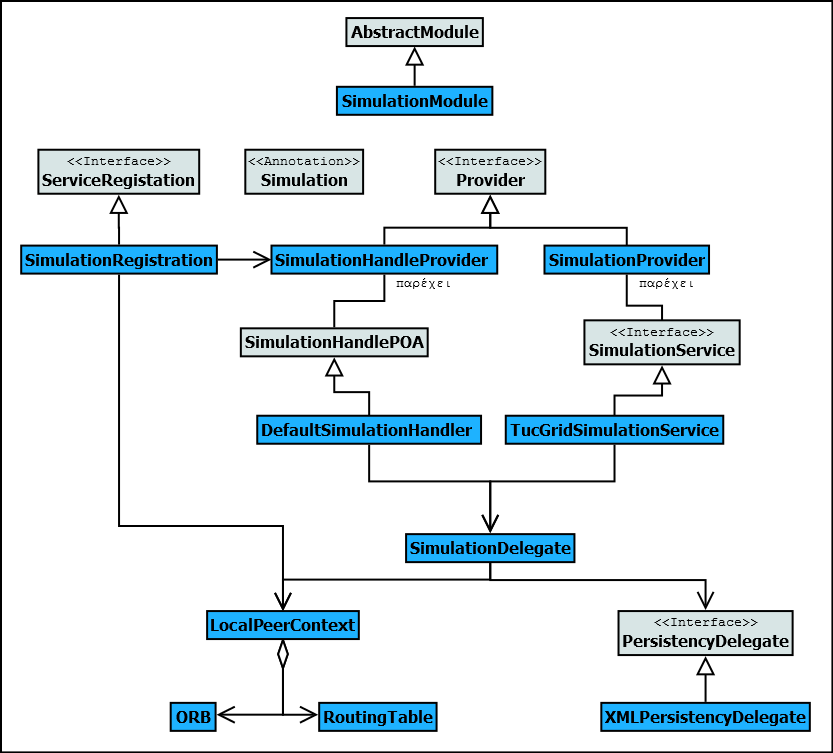
\includegraphics[width=\textwidth]{Figures/Architecture/Service_Layer/SimulationService_ClassDiagram.png}
  \end{center}
  \caption{Διάγραμμα κλάσεων υπηρεσίας Simulation}
  \label{fig:SimulationService}
\end{figure}

Για τον πειραματισμό και τον έλεγχο καλής λειτουργίας του 
συστήματος έχουμε την ανάγκη μιας υπηρεσίας που θα προσφέρει τις 
απαραίτητες λειτουργίες. Αυτό τον σκοπό εξυπηρετεί η υπηρεσία 
προσομοίωσης. 

Η υπηρεσία προσφέρει την διεπαφή SimulationProvider στις διεργασίες και 
στην εφαρμογή. Οι μέθοδοι που προσφέρει είναι:

\newcounter{numberedCntBB}
\begin{enumerate}
\item Ο τερματισμός ενός συγκεκριμένου peer. Ο peer τερματίζει χωρίς να 
ειδοποιήσει το δίκτυο και έτσι προσομοιώνεται μια αποτυχία μέσα στο 
δίκτυο.
\item Η ερώτηση για πληροφορίες ενός peer. Οι πληροφορίες περιλαμβάνουν 
τον πίνακα δρομολόγησης και το μονοπάτι στο οποίο βρίσκεται ο ερωτηθέν 
peer.
\item Ο τερματισμός της προσομοίωσης. Στην ουσία στέλνεται σήμα στο 
δίκτυο και κάθε peer τερματίζει.
\setcounter{numberedCntBB}{\theenumi}
\end{enumerate}
Στην εικόνα \ref{fig:SimulationService} φαίνεται το διάγραμμα κλάσεων 
της υπηρεσίας. Ακολουθείται η ίδια λογική με αυτή της υπηρεσίας Repair.

\subsection{Υλοποίηση Υπηρεσίας Αρχικοποίησης Συστήματος}

\begin{wrapfigure}{L}{0.42\textwidth}
  \begin{center}
    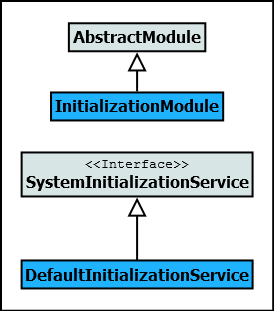
\includegraphics[width=0.40\textwidth]{Figures/Architecture/Service_Layer/InitializationService_ClassDiagram.png}
  \end{center}
  \caption{Διάγραμμα κλάσεων υπηρεσίας αρχικοποίησης}
  \label{fig:InitService}
\end{wrapfigure}

Η Guice κάνει μια μερική αρχικοποίηση του συστήματος μέσω των 
συσχετισμών που υπάρχουν μεταξύ διεπαφών και υλοποιήσεων αλλά δεν είναι 
αρκετή. Η υπηρεσία SystemInitializationService είναι υπεύθυνη για την 
πλήρη αρχικοποίηση του συστήματος. Μέσω της διεπαφής της υπηρεσίας 
μπορούν να ενεργοποιηθούν εκείνες οι υπηρεσίες που είναι απαραίτητες 
στην εφαρμογή. Επίσης, ο τοπικός peer μπορεί να αρχικοποιηθεί σε μια 
προηγούμενη κατάσταση εκτέλεσης της εφαρμογής. Αποθηκεύεται ο πίνακας 
δρομολόγησης σε μορφή XML και κατά συνέπεια μπορεί να φορτωθεί. Τέλος, 
από αυτήν την υπηρεσία ελέγχεται η εκκίνηση και ο τερματισμός της CORBA. 
Στην εικόνα \ref{fig:InitService} φαίνεται το διάγραμμα κλάσεων της υπηρεσίας. 
Παρατηρούμε πως ξεφεύγει από την γενική δομή και ο λόγος είναι απλότητα 
της υπηρεσίας.

\section{Επίπεδο Διαδικασιών - Process Layer}

Όπως αναλύθηκε, μια σημαντική αρχή των υπηρεσιών είναι αυτή της 
σύνθεσης. Μέσω αυτής της σύνθεσης προκύπτουν οι διεργασίες οι οποίες 
ανήκουν στο παρόν επίπεδο. Στην εικόνα \ref{fig:ProcessComponent} φαίνονται 
οι διαδικασίες που περιλαμβάνονται με τις διεπαφές που εκθέτουν καθώς και τις 
εξαρτήσεις από το επίπεδο των υπηρεσιών. Οι υπάρχουσες διαδικασίες είναι 
δυο αυτή της συνάντησης δυο peer και άλλη μια που χρησιμοποιείται στην 
προσομοίωση του συστήματος.

\begin{figure}[htbp]
  \begin{center}
    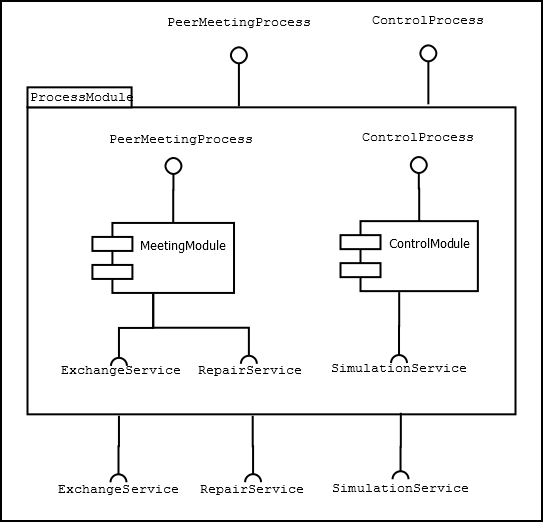
\includegraphics[width=0.6\textwidth]{Figures/Architecture/Process_Layer/Process_ComponentDiagram.png}
  \end{center}
  \caption{Διάγραμμα συστατικών επιπέδου διαδικασιών}
  \label{fig:ProcessComponent}
\end{figure}

\subsection{Διαδικασία Συνάντησης Peer}

\begin{figure}[htbp]
  \begin{center}
    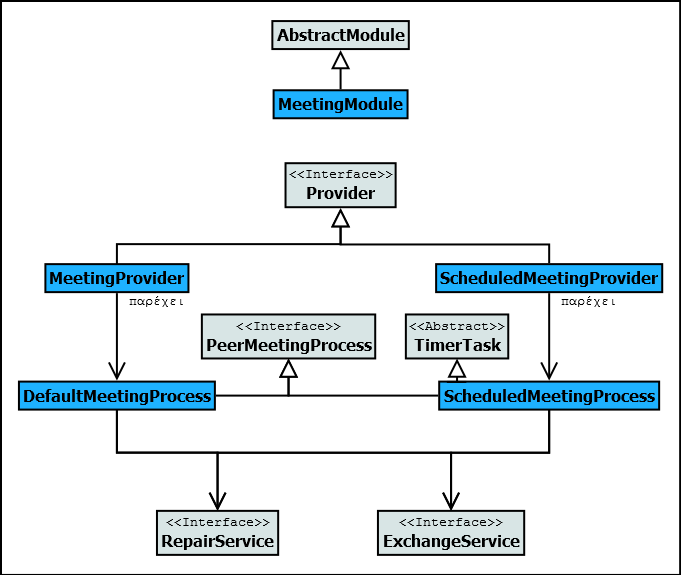
\includegraphics[width=0.9\textwidth]{Figures/Architecture/Process_Layer/MeetingProcess_ClassDiagram.png}
  \end{center}
  \caption{Διάγραμμα κλάσεων διαδικασίας συνάντησης}
  \label{fig:MeetingProcess}
\end{figure}

Η διαδικασία συνάντησης είναι τα βήματα που ακολουθούνται όταν 
ένας peer θέλει να εκτελέσει τον αλγόριθμο exchange. Κατά τον Aberer 
\citep{Abererb} σε κάθε επικοινωνία που γίνεται μεταξύ δυο peer 
εκτελείται ο αλγόριθμος. Τα βήματα που εκτελεί η διαδικασία είναι η 
εκτέλεση της υπηρεσίας ExchangeService και στην περίπτωση που έχουμε 
CommunicationException, δείγμα ότι ο απομακρυσμένος peer έχει αποτύχει, 
εκτελείται η υπηρεσία RepairService για την λύση του προβλήματος.

Η διαδικασία όπως φαίνεται στο διάγραμμα κλάσεων της στην εικόνα 
\ref{fig:MeetingProcess},ακολουθεί την γενική δομή που αναλύθηκε. 
Συγκεκριμένα, ορίζεται και παράλληλα εκτίθεται στο επίπεδο εφαρμογής 
η διεπαφή PeerMeetingProcess. Προσφέρει μια μέθοδο που θέτει σε κίνηση τα βήματα 
όπως περιγράφηκαν στην προηγούμενη παράγραφο.

Έχουμε δυο υλοποιήσεις της διεπαφής. Η πρώτη είναι μια κλασική 
υλοποίηση η οποία προορίζεται να χρησιμοποιηθεί από την εφαρμογή 
καλώντας η ίδια την διαδικασία όποτε θέλει. Η δεύτερη αφορά τον χρονικό 
προγραμματισμό της διεργασίες, ώστε να εκτελείται μετά το πέρας 
συγκεκριμένων χρονικών διαστημάτων. Αυτή επιλέγει τυχαία από τον πίνακα 
δρομολόγησης έναν peer και εκτελεί τη διαδικασία συνάντησης. Για να 
επιτευχθεί αυτό η διαδικασία επεκτείνει την κλάση TimerTask που 
προσφέρει η Java. Στη συνέχεια η εφαρμογή θα πρέπει να δημιουργήσει έναν 
Timer και να εγκαταστήσει την διαδικασία για εκτέλεση.

\subsection{Διαδικασία Ελέγχου Δικτύου}

Η διαδικασία αυτή έχει δημιουργηθεί για τον έλεγχο ενός δικτύου 
PGrid από έναν συγκεκριμένο peer. Αποτελείται από μια κλάση την 
ControlProcess και η λειτουργικότητα που προσφέρει είναι ο εξαναγκασμός 
αποτυχίας ενός peer και η προβολή του μονοπατιού που έχουν όλοι οι peer 
του δικτύου. Να σημειωθεί πως ο peer που είναι υπεύθυνος για τον έλεγχο 
γνωρίζει όλους τους peer του δικτύου.
